\clearpage\section{Chapter 8: Threads}

Threads are the building blocks for concurrent (also known as
{\em parallel\/}) execution. In a concurrent program,  the program
instructions specify multiple things to compute at the same time,
during some or most of the program run.  On a classic single processor
system these computations will only happen one at a time, but on most
modern multiprocessor and multicore systems, the hardware is designed
to do several computations at once, and if your program does not ask
for as much, it is underutilizing (sometimes severely) the platform.

This chapter describes Unicon's concurrency facilities. It is based
on Unicon Technical Report 14 and the implementation work of Jafar
Al Gharaibeh; UTR14 on the unicon.org site may amend this chapter
with added features in future.
Threads are an extension of the co-expression type described in
Chapter 4 and the system interface described in Chapter 5.
Consulting those chapters may be helpful in studying this one.

Concurrent programming introduces techniques, concepts and difficulties
that do not exist in sequential programs. In some situations concurrent
programming is a natural way to write programs, such as a server where
threads serve different clients. In other situations, concurrent
programming improves performance. Long running programs can run faster
by having several threads running cooperatively on several CPU cores in
the system, or programs that do a lot of slow I/O operations can allow
other non-blocked threads to proceed and utilize the CPU. However, for
programs that have a lot of dependencies and are sequential in nature,
the complexities of parallelizing them can outweigh the benefits.

This chapter is not a comprehensive concurrent programming guide. It
assumes that the reader has some basic knowledge about threads, their
programming techniques
and problems, such as synchronization and race conditions. Readers who are
unfamiliar with concurrency can refer to a myriad of resources
such as [Andr83] or [Bute97] for an overview. Since Unicon{\textquoteright}s
concurrency facilities are implemented on top of POSIX threads, many of
the concepts from pthreads programming apply, often with more
concise, or higher-level ways of writing things.

\subsection[Threads and Co{}-Expressions ]{Threads and Co-Expressions}

Co-expressions are independent, explicitly sequential execution contexts.
Only one co-expression is active at any given moment. When
a co-expression is activated, the calling co-expression blocks until
the child co-expression returns the execution to it or fails. Threads
on the other hand, can run simultaneously and independently. Threads
in Unicon are as special co-expressions that are marked to run
asynchronously.

In a concurrent
program that has two or more threads that execute simultaneously
working toward some specific goal, each thread has its own program
counter, stack pointer and other CPU registers. However, all of the
threads in a program share the address space, open files and many other
pieces of process-wide information. This enables very fast
communication and cooperation between threads, which leads to less
blocking, faster execution and more efficient use of resources. 

Unicon programs start execution in the {\texttt main()} procedure. In a
multi-thread programming environment, the procedure {\texttt main()} is
the entry point for a special thread referred to as the
{\em main thread}. This main thread
gets created by the operating system when the program first runs. The
main thread can create new threads which can create even more threads.
\ Each thread has an entry point of execution where the thread first
starts executing. Usually this is a procedure but it can be any Unicon
expression, as is the case for co-expressions. When a thread first
starts running in the entry point, it goes on its own execution path,
separate from the thread that created it, which continues to run. A
thread never returns. When it ends, it simply terminates; other threads
continue to run. An important exception is the main thread; if the main
thread ends, the whole program ends. If there are any other threads
running, all of them will be terminated. 



Since the emergence of the first computer, processors have been
increasing in computational power. Central processing unit speeds grew
faster than almost all of the other units in the computer, especially
the I/O units. This causes programs, especially those which are I/O
bound, to spend most of their execution time blocked waiting for I/O to
complete. On systems with multitasking support, several programs run
at the same time. When one program blocks for I/O for example, another
program is scheduled to run allowing a better utilization of the system
resources. Multitasking offered a way to increase the overall system
throughput and boosted the utilization of the increasingly powerful
computers. Multitasking however, could not help make a process run
faster, even on multiprocessor systems.

\subsection[First Look at Unicon Threads]{First Look at Unicon Threads}

Unicon threads facilities give the programmer flexibility in choosing
the programming styles that suit the problem in hand. In many
situations the same problem can be solved in different ways, using
implicit features or explicit ones. The following sections cover the
functions and features provided by the threads facilities in Unicon.

\subsubsection{Thread Creation}

Threads can be created in two ways in Unicon, using the
\texttt{thread} reserved word or using the function
\texttt{spawn()}. The difference between the two is the
separation between creating a thread and running it. The thread
reserved word creates a thread and starts its execution. The function
\texttt{spawn()} however takes a previously created
co-expression and turns it into a thread. In many cases the thread
reserved word allows more concise code. \texttt{spawn()} on
the other hand is useful in situations where several threads need to be
created and initialized before running them.
\texttt{spawn()} also takes extra optional parameters
to control some aspects of the newly created thread. The following code
creates and runs a hello world thread.

\iconcode{
thread write({\textquotedblleft}Hello World!{\textquotedblright})
}

\noindent This is equivalent to:

\iconcode{
spawn( create write({\textquotedblleft}Hello World!{\textquotedblright}))
}

\noindent or

\iconcode{
co := create write({\textquotedblleft}Hello World!{\textquotedblright}) \\

spawn(co)
}

Both thread and \texttt{spawn()} return a reference to the
new thread. The following program creates 10 threads: 

\iconcode{
procedure main() \\

\ \ \ every i := !10 do thread write({\textquotedblleft}Hello World! I
am thread: {\textquotedblright} , i ) \\

\ \ \ write({\textquotedblleft}main : done{\textquotedblright}) \\

end
}

In this example, the main thread continues to execute normally after
firing 10 threads. Because of the non-deterministic nature of threads,
there is no guarantee which thread gets to print out its hello world
message first, or what order the messages are printed out including the
message from the main thread
\texttt{{\textquotedblleft}}\texttt{main}\texttt{
}\texttt{:}\texttt{
}\texttt{done}\texttt{{\textquotedblright}}\texttt{.}
\ All of the possible permutations are valid. No assumptions can be
made about which one will continue running or finish first. It depends
on the host OS CPU process/thread scheduler. The order is
unpredictable.

Furthermore, the main thread might finish and terminate the program
before some or all of the threads get executed or print out messages.
To avoid such situations, the main thread needs to wait for other
threads to finish before exiting the program. This is can be achieved
using the function \texttt{wait()}, which blocks the calling
thread until the target thread is done. The above program can be
rewritten as the following:

\iconcode{
procedure main() \\

\ \ \ L := [ ] \\

\ \ \ every i := !10 do put(L , thread write({\textquotedblleft}Hello
World! I am thread: {\textquotedblright} , i )) \\

\ \ \ every wait(!L) \\

\ \ \ write({\textquotedblleft}main : done{\textquotedblright}) \\

end
}

\noindent
\texttt{wait(!L)} tells the main the thread to wait for
every thread to finish, causing the message {\textquotedblleft}main :
done{\textquotedblright} to be the last thing printed out before the
program ends. \texttt{wait()} is useful in cases
where threads need to synchronize so that one thread blocks until
another finishes. \texttt{wait()} provides a very basic
synchronization technique, but most concurrent programming tasks
need more synchronization than waiting for a thread to finish.
Advanced synchronization mechanisms are discussed below.


\subsubsection[Thread Evaluation Context]{Thread Evaluation Context}

Similar to co-expressions, threads have their own stack, starting from a
snapshot of parameters and local variables at creation time. This
allows co-expressions and threads to be used outside the scope where
they are created. It also allows a thread to start evaluation using the
values of variables at the time of creating the thread rather than when
running it in the case of \texttt{spawn()}. Another
important side effect of this process is avoiding race conditions
because each thread gets a copy of the variables instead of having all
the threads competing on the same shared variables. Race conditions and
thread safe data will be covered in depth in the following section. The
following example and its output demonstrate the idea of an evaluation
context:

\iconcode{
procedure main() \\

\ \ \ local x:= 10, y:=20, z:=0 \\

\ \ \ write( {\textquotedbl}Main thread: x={\textquotedbl}, x,
{\textquotedbl}, y={\textquotedbl}, y, {\textquotedbl},
z={\textquotedbl},z) \\

\ \ \ thread (x:=100) \& write({\textquotedbl}Thread 1:
x={\textquotedbl}, x) \\

\ \ \ thread (y:=200) \& write({\textquotedbl}Thread 2:
y={\textquotedbl}, y) \\

\ \ \ thread (z:=x+y) \& write({\textquotedbl}Thread 3:
z={\textquotedbl}, z) \\

\ \ \ delay(1000) \\

\ \ \ write( {\textquotedbl}Main thread: x={\textquotedbl}, x,
{\textquotedbl}, y={\textquotedbl}, y, {\textquotedbl},
z={\textquotedbl},z) \\

end
}

\noindent
output:

\iconcode{
Main thread: x=10, y=20, z=0 \\

Thread 3: z=30 \\

Thread 1: x=100 \\

Thread 2: y=200 \\

Main thread: x=10, y=20, z=0 \\
}

\ \ \textit{NOTE: the delay(1000) should give the threads enough time to
run and finish before the main program finishes. Don{\textquoteright}t
leave it to chance: wait() will block until threads finish instead of a
1sec delay. }

The output shows that the changes to the variables are per thread and
are not visible in the main thread or in the other threads. Local
variables{\textquoteright} copies in different threads can be thought
of as passing parameters by value to a procedure. This is true for
local variables of immutable data types; global variables and mutable
types such as lists on the other hand are shared. Any change in the
structure of such types is visible across all threads. Contrast the
following example with the one above:

\iconcode{
procedure main() \\

\ \ \ local L \\

\ \ \ L := [20, 10, 0] \\

\ \ \ write( {\textquotedbl}Main thread: L[1]={\textquotedbl}, L[1],
{\textquotedbl}, L[2]={\textquotedbl}, L[2], {\textquotedbl},
L[3]={\textquotedbl},L[3]) \\

\ \ \ thread (L[1]:=100) \& write({\textquotedbl}Thread 1:
\ L[1]={\textquotedbl}, L[1]) \\

\ \ \ thread (L[2]:=200) \& write({\textquotedbl}Thread 2:
\ L[2]={\textquotedbl}, L[2]) \\

\ \ \ thread (L[3]:=L[1]+L[2]) \& write({\textquotedbl}Thread 3:
\ L[3]={\textquotedbl}, L[3]) \\

\ \ \ delay(1000) \\

\ \ \ write( {\textquotedbl}Main thread: L[1] ={\textquotedbl}, L[1],
{\textquotedbl}, L[2]={\textquotedbl}, L[2], {\textquotedbl},
L[3]={\textquotedbl},L[3]) \\

end
}

\noindent
output:

\iconcode{
Main thread: L[1]=20, L[2]=10, L[3]=0 \\

Thread 2: \ L[2]=200 \\

Thread 3: \ L[3]=300 \\

Thread 1: \ L[1]=100 \\

Main thread: L[1] =100, L[2]=200, L[3]=300 \\
}

\noindent
Instead of using three variables \texttt{x},
\texttt{y} and \texttt{z}, a list of size three
is used. \texttt{x} from the previous example maps to
\texttt{L[1]}, \texttt{y} to
\texttt{L[2]}, and z to \texttt{L[3]}. The
program does the same thing as before, but any
change to the content of \texttt{L} is visible in other
threads. Unlike the output in the first case where the values of
\texttt{x}, \texttt{y}, and \texttt{z}
remained the same in the main thread, the output in the second example
shows that the changes to the list elements in the other threads were
visible in the main thread.

\subsubsection[Passing Arguments to Threads]{Passing Arguments to
Threads}

When creating a new thread for a procedure, the parameters that are
passed to the procedure at thread creation time can be thought of as a
one-time one-way communication between the creator thread and the new
thread. This is very useful in initializing the new thread or passing
any data that thread is supposed to work on. The following program has
three threads in addition to the main thread. The main thread passes a
list to each thread which in turn calculates the summation of the list
elements and prints it out to the screen:

\iconcode{
procedure main() \\
\>   L1 := [1, 2, 3] \\
\>   L2 := [4, 5, 6] \\
\>   L3 := [7, 7, 9] \\
\>   t1 := thread sumlist(1, L1) \\
\>   t2 := thread sumlist(2, L2) \\
\>   t3 := thread sumlist(3, L3) \\
\>   every wait(t1{\textbar}t2{\textbar}t3) \\
end \\
\ \\
procedure sumlist(id, L) \\
\>   s := 0 \\
\>   every s +:= !L \\
\>   write({\textquotedbl} Thread id={\textquotedbl}, id,
{\textquotedbl} result={\textquotedbl}, s) \\
end
}

\noindent
output:

\iconcode{
\ Thread id=2 result=15 \\

\ Thread id=1 result=6 \\

\ Thread id=3 result=23
}

Since the lists are independent, there are no chances of a race
condition. The example shows that the second thread was the first to
finish and print out its result. If the problem solution requires
sharing data or guaranteeing that one thread should finish before
another thread, then a synchronization mechanism should be used. This
is the subject of the next section.

\subsection[Thread Synchronization]{Thread Synchronization}

Thread synchronization can be done in many different ways. Some problems
require more synchronization than others. Some may require using
advanced synchronization mechanisms and rely on the language support to
achieve full control over the execution of threads and protect shared
data. This section covers many synchronization techniques in the Unicon
language and also introduces the concept of race condition in a
multi-thread environment, and thread safe code.

\subsubsection[The Non{}-Deterministic Behavior of Threads ]{The
Non-Deterministic Behavior of Threads }

Programming with threads introduces a whole new set of concepts and
challenges that non-threaded programs do not have to deal with. \ In
most multi-threaded programs, threads need to communicate through
shared data. Because threads run in different non-deterministic order
they access and update shared data in a non-deterministic fashion.
Consider the following popular example where two threads try to
increment a shared variable called \texttt{x} whose initial
value is \texttt{0}.

\ \ \ \ \textit{Thread}\textit{ }\textit{1\ \ \ \ \ \ Thread2}\textit{
}\textit{\ \ \ \ }

\ \ \ \ x:=x+1
\ \ \ \ \ \ \ \ \ \ \ \ \ \ \ \ \ \ \ \ \ \ \ \ \ \ \ \ \ \ \ \ \ \ \ \ \ \ \ x:=x+1
\ \ \ \ \ \ \ \ \ \ \ \ \ \ \ \ \ \ \ \ \ \ 

While \texttt{x:=x+1} does not look like it would make a
problem, in reality it does. This happens because
\texttt{x:=x+1} is not atomic. In many computer systems this
can be broken down to three operations: fetch the value of
\texttt{x}, increment \texttt{x} and then store
the new value back in \texttt{x}. These three
operations might occur at different times in different threads.
\textit{Thread}\textit{ }\textit{2} for example might fetch
\texttt{x}, followed by \textit{Thread}\textit{
}\textit{1} also fetching it but before \textit{Thread 2} stores back
the new value of \texttt{x}, leaving \textit{Thread 1
}working on the old value of \texttt{x}. \textit{Thread
1 }should not be allowed to read the value of
\texttt{x} in the middle of an operation where another
thread is updating the value of the variable. \ Consider the following
scenarios, starting with \ \texttt{x:=0}\texttt{
}


\bigskip

Scenario 1

\textit{\ \ \ \ }\textit{Thread}\textit{
}\textit{1}\textit{\ \ \ \ \ \ }\textit{Thread 2}\textit{
}\textit{\ \ }\ \ 

\ \ \ \ \ fetch x \ (0)
\ \ \ \ \ \ \ \ \ \ \ \ \ \ \ \ \ \ \ \ \ \ \ \ \ \ \ \ \ \ fetch x (0)

\ \ \ \ \ increment x (1)
\ \ \ \ \ \ \ \ \ \ \ \ \ \ \ \ \ \ \ \ \ \ \ increment x (1)
\ \ \ \ \ \ \ \ \ \ \ \ \ \ \ \ \ \ \ 

\ \ \ \ \ store x \ \ (1)
\ \ \ \ \ \ \ \ \ \ \ \ \ \ \ \ \ \ \ \ \ \ \ \ \ \ \ \ store \ x (1)
\ 

\ \ \ {}-{}-{}-{}-{}-{}-{}-{}-{}-{}-{}-{}-{}-{}-{}-{}-{}-{}-{}-{}-{}-{}-{}-{}-{}-{}-{}-{}-{}-{}-{}-{}-{}-{}-{}-{}-{}-{}-{}-{}-{}-{}-{}-{}-{}-{}-{}-{}-{}-{}-{}-{}-{}-{}-{}-{}-{}-{}-{}-{}-{}-{}-{}-{}-{}-{}-{}-{}-
The final value of \texttt{x} is \texttt{1}


\bigskip

Scenario 2

\textit{\ \ \ \ }\textit{Thread}\textit{
}\textit{1}\textit{\ \ \ \ \ \ }\textit{Thread 2}\textit{
}\textit{\ \ \ \ }

\ \ \ \ \ fetch x \ (0) \ \ \ \ \ \ \ \ \ \ \ \ \ \ \ \ \ \ \ \ \ \ \ \ 

\ \ \ \ \ increment x (1) \ \ \ \ \ \ \ \ \ \ \ \ \ \ \ \ \ 

\ \ \ \ \ store x \ \ (1) \ \ \ \ \ \ \ \ \ \ \ \ \ \ \ \ \ \ \ \ \ \ \ 

\ \ \ \ \ \ \ \ fetch x (1)

\ \ \ \ \ \ \ \ increment x (2)

\ \ \ \ \ \ \ \ store x \ \ (2)

\ \ \ {}-{}-{}-{}-{}-{}-{}-{}-{}-{}-{}-{}-{}-{}-{}-{}-{}-{}-{}-{}-{}-{}-{}-{}-{}-{}-{}-{}-{}-{}-{}-{}-{}-{}-{}-{}-{}-{}-{}-{}-{}-{}-{}-{}-{}-{}-{}-{}-{}-{}-{}-{}-{}-{}-{}-{}-{}-{}-{}-{}-{}-{}-{}-{}-{}-{}-{}-{}-{}-
The final value of \texttt{x} is \texttt{2}


\bigskip

In Scenario 1 the final value of \texttt{x} is
\texttt{1}, even though there are two increments done by the
two threads. In Scenario 2 however the final value is
\texttt{2}. This unpredictable outcome does not necessarily
mean a problem or a bug that must be handled. \ Non-deterministic
execution is part of multi-threaded programming culture that many
programs can live with. For example, if one or more threads depend on a
counter to update the screen every 100 increments or so, but it does
not need to be exactly 100 increments, then the threads can increment
the counter without worrying about a race condition or synchronizing
access to the shared counter. If deterministic execution must be
guaranteed, programmers have to take extra steps to ensure a specific
order and predictable results. That is where thread synchronization
comes into play.

\subsubsection[User Defined Synchronization]{User Defined
Synchronization}

For some simple situations, synchronization can be achieved without
relying on special synchronization primitives provided by the language.
For example, if one thread is waiting for another thread to finish a
task, a shared flag variable can be used in such case. In the following
example, the main thread might finish before the child thread:

\iconcode{
procedure main() \\
\>   thread \ write({\textquotedbl}I am a thread: Hello
World!{\textquotedbl}) \\
end
}

As seen in the previous section, this can be handled using the
\texttt{wait()} function or \texttt{delay()}. The
\texttt{wait()} function is the best solution for this
situation. The function \texttt{delay() }works but there are
two problems associated with it: it forces the program to wait a lot
longer than necessary, and second, if the delay time is not long enough
and depending on the system, the main thread might still finish before
the child thread. Actually even with a long delay, there is no
guarantee the child thread would be done. In a real application,
\texttt{delay()} would be a poor choice. Here is an
alternative solution other than using \texttt{wait()}:

\iconcode{
global done \\
procedure main() \\
\ \ \ thread \ (write({\textquotedbl}I am a thread: Hello
World!{\textquotedbl}) \& done:={\textquotedbl}true{\textquotedbl}) \\
\ \ \ until {\textbackslash}done \\
end
}

In this case, the loop \texttt{until
{\textbackslash}}\texttt{done} ensures that the main thread
keeps spinning until the child thread set the variable
\texttt{done} to a non-null value. It avoids the problems
with using delay(), at the expense of burning up 100\% of one CPU in a
spin-lock. Note that declaring \texttt{done} to be global is
a key for the example above to work. If it were local, the main thread
would spin indefinitely and never finish! That is because any change to
\texttt{done} in the child thread would be invisible in the
main thread. If none of these approaches seems acceptable, that is a
good sign. Use techniques from the following sections to avoid such
inefficient synchronization.

\subsubsection[Language Support for Synchronization]{Language Support
for Synchronization}

Using function \texttt{wait()} or global variables to synchronize between
threads might be sufficient in some situations, but most problems require
more efficient synchronization methods, enabled by mutexes and condition
variables.

\paragraph{Critical Regions and Mutexes}
A \textit{mutex} (from mutual exclusion) is a synchronization
object used to protect shared data and serialize threads in
\textit{critical regions}, sequences of instructions in which only
one thread may execute at a time or an error will occur. In the example
discussed at the beginning of this chapter, two threads compete
to increment the variable \texttt{x}. The end result might not be what the
programmer intended. In such cases a mutex may be used to protect
access to the variable \texttt{x}. Any operation (including
data structure traversal) where more than one thread can execute
non-deterministically, leading to data corruption or incorrect results
is called \textit{thread unsafe}. Thread unsafe code or data
structures have to be handled correctly via synchronizations mechanisms
to achieve correct behavior with correct results.

A mutex object is created using the \texttt{mutex()}
function. The returned mutex object can be locked/unlocked via the
functions \texttt{lock()} and \texttt{unlock()}
to serialize execution in a critical region. The following example
demonstrates the use of a mutex to protect increments to the global
variable \texttt{x}:

\iconcode{
global x \\
procedure main() \\
\>   mtx\_x := mutex() \\
\>   x := 0 \\
\>   t1 := thread inc\_x(mtx\_x) \\
\>   t2 := thread inc\_x(mtx\_x) \\
\>   every wait(t1 {\textbar} t2) \\
\>   write({\textquotedbl}x={\textquotedbl}, x) \\
end \\
\ \\
procedure inc\_x(region) \\
\>   lock(region) \\
\>   x := x + 1 \\
\>   unlock(region) \\
end
}

It is important to note that the mutex object has to be initialized only
once and can then be shared between all of the threads
(\texttt{t1} and \texttt{t2}) accessing
the critical region (\texttt{x := x + 1}).
\texttt{lock(region)} marks the beginning of the
critical region protected by the mutex region.
\texttt{unlock(region)} marks the end of the critical
region. When a thread calls \texttt{lock(region)}, it
tries to acquire the mutex \texttt{region}. If
\texttt{region} is not
{\textquotedblleft}owned{\textquotedblright} by any other thread,
\texttt{lock(region)} succeeds and the thread becomes
the owner of the mutex \texttt{region} and then enters
the critical region, otherwise the thread blocks until the current
owner of the mutex leaves the critical region by calling
\texttt{unlock(region)}. Since there are two threads
and \texttt{x:=x+1} is protected by a mutex, the output of
the program is guaranteed to be \texttt{x=2}, unlike the
case where a mutex is not used, in which case \texttt{x=1}
or \texttt{x=2} are viable outputs.

The more critical-regions/mutexes a concurrent program has, the slower
it runs. The length of the critical region also affects the
performance. The longer the critical region, the more time it takes a
thread to finish the critical region and release the mutex, which
increases the probability that other threads become blocked waiting to
acquire the mutex and enter the critical region. Locking a mutex and
forgetting to unlock it is very likely to lead to a deadlock, a common
problem in concurrent programming, where all threads block waiting for
each other, and for resources to become available. Because all threads
are blocked, resources will not be freed, and the threads block
indefinitely. 

Unicon provides a special syntax for critical regions
equivalent to a \texttt{lock()}/\texttt{unlock()}
pair, that aims mainly to guarantee that a mutex is released at the end
of a critical region, beside enhancing the readability of the program.
Here is the syntax:

\iconcode{
critical mtx: expr
}

\noindent
This is equivalent to:

\iconcode{
lock(mtx) \\
expr \\
unlock(mtx)
}

Given a global variable named \texttt{region} that has
been initialized as a mutex, the code to increment
\texttt{x} in the previous example can be written as:

\iconcode{
critical region: x := x + 1
}

The critical region syntax only unlocks the mutex if it executes to
the end. If there is a \texttt{return} or \texttt{break} in the critical region
body, then it is the programmer{\textquoteright}s
responsibility to explicitly unlock the mutex of the critical region.
For example:

\iconcode{
critical region: \{ \\
\>   if x {\textgreater} 100 then \{ unlock(region); return \} \\
\>   x := x + 1 \\
\>   \}
}

In some situations, a thread might have several tasks to finish and may
not want to block waiting for a mutex that is possessed by another
thread. For example, if a thread is creating items that can be inserted
in one of several shared queues, the thread can insert every new item
in the first queue that it acquires. \texttt{trylock()}
is an alternative function for \texttt{lock()}. The
only difference is that \texttt{trylock()} is
non-blocking. If the thread cannot acquire the mutex immediately, the
function fails. The most suitable way to use
\texttt{trylock()} is to combine it with an
\texttt{if} statement, where the
\texttt{then} body unlocks the mutex after finishing
the work on the protected object as follows:

\iconcode{
if trylock(mtx) then \{ \\
\ \ \ \ \ expr \\
\ \ \ \ \ unlock(mtx) \\
\ \ \ \ \ \}
}

Both \texttt{lock()} and \texttt{trylock()}
return a reference to the mutex or the object they acquired (upon
succeeding in case of \texttt{trylock()}). This makes
it very convenient to write code like the following assuming L1 and L2
are both lists that are marked as shared:

\iconcode{
item := newitem() \\
if L := trylock(L1 {\textbar} L2) then \{ \\
\ \ \ \ \ put(L, item) \\
\ \ \ \ \ unlock(L) \\
\ \ \ \ \ \}
}

Note that trylock() may fail to lock any of the lists leaving item
unprocessed. Depending on what the code needs to do, if it is required
to guarantee that it does not proceed before one of the locks to
\texttt{L1} or \texttt{L2} succeeds
then it can be written as follows:

\iconcode{
item := newitem() \\
until L := trylock(L1 {\textbar} L2) \\
put(L, item) \\
unlock(L)
}

\paragraph[Initial clause]{Initial clause}
A procedure in a Unicon program can have an initialization clause at the
top of the procedure. This gets executed only once the first time the
procedure is entered. The initial clause provides a very convenient way
to place local static variables and their initialization in the same
procedure instead of relying on global variables and having to
initialize them somewhere else. A procedure that produces a sequence of
numbers one at each call can be written as:

\iconcode{
procedure seq() \\
\ \ \ static i \\
\ \ \ initial i := 0 \\
\ \ \ i := i + 1 \\
\ \ \ return i \\
end
}

Initial clauses are thread-safe. They can be thought of as a built-in
critical region that is run only once. No thread is allowed to enter
the procedure if there is a thread currently still executing in the
initial block. This can be useful specifically in a concurrent
environment to do critical initialization such as creating a new mutex
object instead of declaring a mutex variable to be global and
initializing it somewhere else or passing it from one function to
another where it will be actually used. A concurrent version of
\texttt{seq()} would look like this:

\iconcode{
procedure seq() \\
\ \ \ local n \\
\ \ \ static i, region \\
\ \ \ initial \{ i:=0; region:=mutex() \} \\
\ \ \ critical region: n := i := i + 1 \\
\ \ \ return n \\
end
}

With the use of the initial clause, \texttt{seq()} is
self-contained and thread safe. Note the use of the local variable
\texttt{n} to temporarily hold the value of the counter
\texttt{i} while still in the critical region. That is
because once the thread leaves the critical region, there is no
guarantee that the value of \texttt{i} would remain the same
before returning the value of \texttt{i}. Using the variable
\texttt{n} guarantees that the value returned is correct
even if the value of \texttt{i} is changed by another
thread.

\paragraph[Thread{}-safe Data Structures]{Thread-safe Data Structures}
In Unicon, mutexes are not just independent objects as described above,
mutexes are also attributes of other objects, namely attributes of the
mutable data types. Any data structure in Unicon that can be used in a
thread unsafe manner can be protected by turning on its mutex
attribute. Instead of declaring a separate mutex, locking and unlocking
it, the structure can just be marked as {\textquotedblleft}needs a
mutex/protection{\textquotedblright} and the language does an implicit
locking/unlocking, protecting the operations that might affect the
integrity of the data structure. For example, if several threads are
pushing and popping elements into and out of a list, this creates
thread-unsafe operations on the list that require protection. \ The
value of implicit mutexes is made clear after considering the
alternative. The following producer-consumer example uses a list to
send and receive data and protects it using an explicit mutex: 

\iconcode{
procedure main() \\
\ \ \ L := [ ] \\
\ \ \ mtx := mutex() \\
\ \ \ p := thread produce(L, mtx) \\
\ \ \ c := thread consume(L, mtx) \\
\ \ \ every wait(p {\textbar} c) \\
end \\
\ \\
procedure produce(L, region) \\
\ \ \ every i := !10 do \\
\ \ \ \ \ \ critical region: put(L, i) \\
end
\ \\
procedure consume(L, region) \\
\> i := 0 \\
\> while i {\textless} 10 \ do \\
\> \> critical region: if x := get(L) then i +:= 1 \& write(x) \\
end
}

Using a thread-safe list results in less lines of code to do the same
thing and also produces a more efficient program doing less locking and
unlocking at the language level, or even not doing explicit locking at
all. For example, the program above may be rewritten as the following: 

\iconcode{
procedure main() \\
\ \ \ L := mutex([ ]) \\
\ \ \ p := thread produce(L) \\
\ \ \ c := thread consume(L) \\
\ \ \ every wait(p {\textbar} c) \\
end \\
\ \\
procedure produce(L) \\
\ \ \ every put(L, !10) \\
end
\ \\
procedure consume(L) \\
\ \ \ i := 0 \\
\ \ \ while i {\textless} 10 \ do \\
\ \ \ \ \ \ if x := get(L) then i +:= 1 \& write(x) \\
end
}

The \texttt{produce()} and \texttt{consume()}
\ procedures do not do any locking, making concurrent programming in
such a case just as easy as writing a sequential program. The only
needed step is notify the language at the beginning that the data
structure is shared, by passing it to the \texttt{mutex()}
function. The \texttt{mutex()} function takes a second
optional parameter denoting an existing mutex object or an object that
is already marked as shared (has a mutex attribute). Instead of
creating a new mutex object for the data structure, the existing mutex
is used as an attribute for the data structure. If the second object is
a structure that is not marked as shared, a new mutex is created. This
is useful when two objects needs to be protected by the same mutex. For
example, the list \texttt{L} and the table
\texttt{T} in the following example share the same mutex:

\iconcode{
mtx := mutex() \\
L := mutex([ ], mtx) \\
T := mutex(table(), mtx)
}

which is equivalent to the following if the mutex does not need to be
explicit:

\iconcode{
L := mutex([ ]) \\
T := mutex(table(0), L)
}

or

\iconcode{
L := [ ] \\
T := mutex(table(0), L)
}

In all cases, \texttt{lock(L)} and
\texttt{lock(T)} lock the same mutex, serializing execution
on both data structures. Not all operations on data structures produces
correct results, only {\textquotedblleft}atomic{\textquotedblright}
operations do. In other words, implicit locking/unlocking takes place
per operation, which means even if each one of the two operations is
safe, the combination might not be. A critical region is still needed
to combine the two. For example, if
\texttt{L}\texttt{[1]} has the value of 3 and two
threads are trying to increment \texttt{L[1]}:

\iconcode{
L[1] := L[1] + 1
}

the result in \texttt{L[1]} could be 4 or 5. That is because
reading \texttt{L[1]} (the right side of the assignment) and
storing the result back in \texttt{L[1]} are two different
operations (not atomic) and are actually separated in time. The good
news is that solving such an issue does not require an extra explicit
mutex. If \texttt{L} is marked as shared (passed to the
\texttt{mutex()} function ) it can be passed to
\texttt{lock()}/\texttt{unlock()} functions. It
can be used with the critical syntax like the following: \ 

\iconcode{
critical L: L[1] := L[1] + 1
}

\paragraph[Condition variables]{Condition variables}
Mutexes are used to protect shared data in critical regions, and block
threads if there is more than one thread trying to enter the critical
region. Condition variables take thread blocking/resumption to a new
level that is not tied to accessing shared data like a mutex. A
condition variable allows a thread to block until an event happens or a
condition changes. For example, the previous section showed a
producer/consumer problem where the consumer keeps spinning to get
values out of the shared list. In similar situations in real life
applications, any spinning could be a waste of resources; other threads
including producer threads could be using the resources doing something
useful instead. The consumer needs to block until there is data to
process in the list. This is where a condition variable comes into
play. \ A condition variable is created using the function
\texttt{condvar()}. The return object is a condition
variable that can be used with \texttt{wait()} and
\texttt{signal()} functions. \texttt{wait(cv)}
blocks the current thread on the condition variable
\texttt{cv}. The thread remains blocked until another
thread does a \texttt{signal(cv)}, which wakes up one thread
blocked on \texttt{cv}. A very important aspect of
using a condition variable is that the condition variable must always
be associated with a mutex. More specifically, the
\texttt{wait()} function has to be always protected by a
mutex. Unicon provides a built-in mutex for condition variables which
can be thought of as an attribute similar to thread safe data
structures. This means a condition variable can also be used with
\texttt{lock()}/\texttt{unlock()} functions or
the critical clause. It is important to realize that not only
\texttt{wait()} has to be protected by a critical region,
but also the condition or the test that leads a thread to wait on a
condition variable. \ See the following example:

\iconcode{
if x=0 then wait(cv)
}

A thread wants to wait on \texttt{cv} if
\texttt{x=0}, but what happens if the value of
\texttt{x} has changed between the test and the call to
\texttt{wait(cv)}? If a second thread changes the value of
\texttt{x} and signals \texttt{cv} \ to wake up
the first thread, while the first thread transitions from the test to
\texttt{wait()}\texttt{,} it ends up missing the
wake up signal and might block indefinitely because it is waiting on a
condition variable that it should not wait on. \ The correct way to use
\texttt{wait()} with a condition variable becomes:

\iconcode{
lock(cv) \\
\ \ \ if x=0 then wait(cv) \\
unlock(cv)
}

or :

\iconcode{
critical cv: if x=0 then wait(cv)
}

Because other threads might need to access the condition variable while
some threads are waiting on it, the \texttt{wait()} function
atomically blocks the thread and releases its corresponding mutex.
After receiving a wake up signal, the blocked thread wakes up, acquires
the mutex (blocking if necessary) and continues executing and that is
when \texttt{wait()} returns. It is a good practice to do
the condition variable test before assuming that it is in one state or
another. This leads to a more correct way to use condition variables
that ensures that a thread does not leave \texttt{wait()}
before guaranteeing the test is in a specific state as follows:

\iconcode{
\ critical cv: while x=0 do wait(cv)
}

Using a \texttt{while} in place of \texttt{if}
will ensure the thread goes back to sleep if the thread happens to wake
up and the condition outcome has not changed.

The producer/consumer example mentioned above can be rewritten using a
condition variable. Since the consumer needs to sleep/wake up depending
on the availability of elements in the list (the list state in other
words), the state of the list needs to be guaranteed to remain the same
while interacting with the condition variable for the same reason
explained above (missing wake up signals). The list and the condition
variable have to be protected by the same mutex.
\texttt{condvar()} allows an optional argument that refers
to an existing mutex to be associated with the condition variable. In
the original example, using an independent mutex to protect the
condition variable looks like this:

\iconcode{
procedure main() \\
\ \ \ L := [ ] \\
\ \ \ mtx := mutex() \\
\ \ \ cv := condvar(mtx) \\
\ \ \ p := thread produce(L, cv) \\
\ \ \ c := thread consume(L, cv) \\
\ \ \ every wait(p {\textbar} c) \\
end \\
\ \\
procedure produce(L, cv) \\
\ \ \ every i := !10 do \{ \\
\ \ \ \ \ \ critical cv: put(L, i) \\
\ \ \ \ \ \ if *L=1 then signal(cv) \\
\ \ \ \ \ \ \} \\
end \\
\ \\
procedure consume(L, cv) \\
\ \ \ i := 0 \\
\ \ \ while i {\textless} 10 \ do \{ \\
\ \ \ \ \ \ if *L=0 then critical cv: until *L{\textgreater}0 do
wait(cv) \\
\ \ \ \ \ \ if x := get(L) then i +:= 1 \& write(x) \\
\ \ \ \ \ \ \} \\
end
}

Another way to implement this program is built on top of the thread safe
list example. Since there is no explicit mutex to pass to the
\texttt{condvar()} function in the original example, a mutex
can be first created and then passed along with the list to the
\texttt{mutex()} function. The same mutex then can be passed
to \texttt{condvar()}. The function binds the mutex already
associated with the list to the condition variable. The final result is
the same as the explicit mutex example, a list and a condition variable
sharing the same mutex. Here is the example again with the shared list
and a condition variable:

\iconcode{
procedure main() \\
\ \ \ mtx := mutex() \\
\ \ \ L := mutex([], mtx) \\
\ \ \ cv := condvar(mtx) \\
\ \ \ p := thread produce(L, cv) \\
\ \ \ c := thread consume(L, cv) \\
\ \ \ every wait(p {\textbar} c) \\
end \\
\ \\
procedure produce(L, cv) \\
\ \ \ every put(L, !10) \& *L=1 \& signal(cv) \\
end \\
\ \\
procedure consume(L, cv) \\
\>   i := 0 \\
\>   while i {\textless} 10 \ do \\
\> \>    if x := get(L) then \\
\> \> \>    i +:= 1 \& write(x) \\
\> \>    else \\
\> \> \>    critical cv: until *L{\textgreater}0 do wait(cv) \\
end
}

In previous examples, calls to \texttt{signal()} are not
protected by any mutex. \texttt{signal()} does not need
protection, because it does not block the thread, and hence there is no
worry about causing a deadlock. The worst thing that can happen is
signaling a condition variable that does not have any thread waiting on
it, which is not a problem. However protecting calls to
\texttt{signal()} is not a problem either. Depending on the
problem, doing it one way or the other might be more or less efficient.
There is no need to have a thread that spends a lot of time
locking/unlocking a mutex if it is not necessary, creating contention
in the critical region. However, a thread that keeps wasting time
signaling condition variables that have no threads waiting on them is
also undesirable.

The \texttt{signal()} function takes a second optional
parameter denoting the number of threads to be woken up. By default,
that number is one, but it can be any positive value. From example:

\iconcode{
every !4 do signal(cv)
}

can be written as:

\iconcode{
signal(cv, 4)
}

Furthermore, if all of the threads waiting on
\texttt{cv} need to be woken up, a special
\texttt{0} ( or \texttt{CV\_BROADCAST})
value can be passed to \texttt{signal()} causing it to
broadcast a wakeup call for all threads waiting on
\texttt{cv}:

\iconcode{
signal(cv, 0)
}

or

\iconcode{
signal(cv, CV\_\texttt{ BROADCAST})
}


\subsection{Thread Communication}


Traditionally, co-expressions communicate implicitly, or explicitly
using the \texttt{@} operator. All co-expression
communication is synchronous; at the two ends of the communication, the
calling co-expression is blocked and the called co-expression runs.
This simple communication model is called \textit{activation} in
Unicon. A co-expression \texttt{C1} can activate another
co-expression \texttt{C2} using the following syntax:

\ x@C2

\texttt{x} is an optional value to be transmitted from
\texttt{C1} to \texttt{C2}.
\texttt{C1} waits until it gets activated by
\texttt{C2} or any other co-expression directly or
indirectly activated by \texttt{C2}. As mentioned earlier,
implicit activation takes place whenever a co-expression produces a
value or falls off its end. With implicit activation, the co-expression
activates its parent (the last co-expression to activate it).

Threads take communication to a completely new level with their dynamic
nature. Threads run concurrently; in many cases, a running thread just
wants to send a value to another thread without waiting for a reply, or
receive a value from another thread if there is one without waiting.
The \texttt{@} operator is not suitable for this kind of
(asynchronous) communication. Unicon adds four operators dedicated for
asynchronous communication. These are
\texttt{@{\textgreater}},
\texttt{@{\textgreater}{\textgreater}},
\texttt{{\textless}@} and
\texttt{{\textless}{\textless}@}. The operators correspond
to send, blocking send, receive and blocking receive.

\subsubsection{Thread Messaging Queues}

Before presenting the communication operators and how they are used, it
is first appropriate to look at messaging queues and how they are
utilized to support the communication model between threads in Unicon.
Each thread maintains two queues called the inbox and outbox that are
created with the thread. When a thread sends a message with an explicit
destination, the message is queued in the destination{\textquoteright}s
inbox. Otherwise, it is queued into the sender{\textquoteright}s outbox.
A thread can receive messages from another thread by dequeuing messages
from the source{\textquoteright}s outbox if there is an explicit
source, otherwise it dequeues messages from its own inbox.  Figure 8-1
presents two threads with the inboxes and outboxes.

\bigskip


\begin{center}
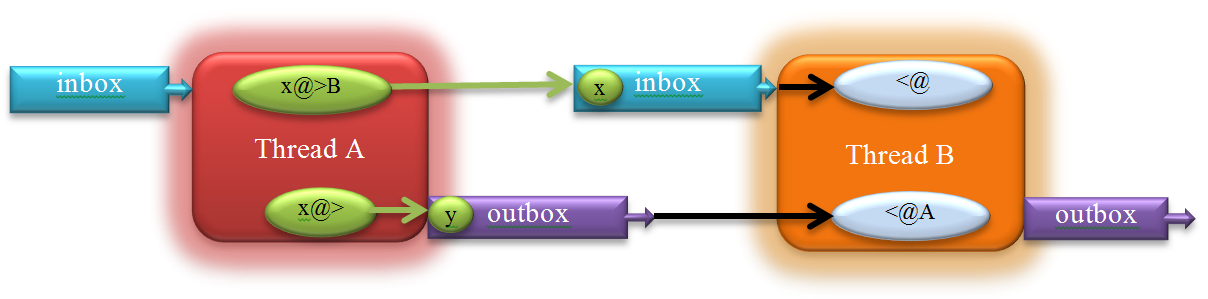
\includegraphics[width=5.75in,height=1.45in]{ub-img/thread-fig1.png}
\end{center}
\vspace{-0.25cm}{\sffamily\bfseries Figure 8-1:}
{\sffamily Inboxes and Outboxes for Thread Communication.}

\bigskip

\subsubsection{Send and Receive Operators}

The first two operators are \texttt{@{\textgreater}} (send)
and \texttt{{\textless}@} (receive). These operators
communicate messages containing arbitrary data between threads. The
operators support co-expressions as well, with the same semantics. The
send operator has the syntax 

\iconcode{
x @{\textgreater}T
}

\texttt{x} can be any data type including null which is
equivalent to omitting it. \texttt{T} refers to a thread to
which \texttt{x} is transmitted. \texttt{X} is
placed in \texttt{T}{\textquoteright}s inbox.
\texttt{X} can be picked by \texttt{T} using the
receive operator which is presented later. The send operator can also
have no destination such as:

\iconcode{
x @{\textgreater}
}

In this case \texttt{x} is sent to no one, instead it is
placed in the sender{\textquoteright}s outbox. The operator can be read
as {\textquotedblleft}produce
\texttt{x{\textquotedblright}}. \texttt{x} can
then be picked later by any thread wanting a value from this sender.
For example the sender thread in this case might be a thread creating
prime numbers and placing them in its outbox to be ready for other
worker threads.

The receive operator is symmetric to the send operator and takes two
forms, with explicit source or with no source as follows:

\iconcode{
{\textless}@T \\
\ \\
{\textless}@
}

The first case reads: receive a value from T, which gets a value from
\texttt{T}{\textquoteright}s outbox, a value produced by
\texttt{T}. Going back to the prime number example mentioned
above, \texttt{{\textless}@T} would be the way to pick a
prime number produced by the prime number generator thread
\texttt{T}. \texttt{{\textless}@} on the other
hand reads values directly from the receiver{\textquoteright}s inbox.
It reads messages sent explicitly to the thread doing the receive
operation.

Both \texttt{@{\textgreater}} and
\texttt{{\textless}@ }can succeed or fail. In the case
of \texttt{{\textless}@} the operator succeeds and
returns a value from the corresponding queue (inbox/outbox) depending
on the operand if the queue is not empty. If the queue is empty the
operation fails directly. In the case of
\texttt{@{\textgreater}}, if the value is placed in the
corresponding queue the operation succeeds and returns the size of the
queue. If the queue is full, the send operation fails. The inbox/outbox
for each thread is initialized to have a limited size (it can hold up
to 1024 values by default). This limit can be increased or decreased
depending on the application needs. The limits are useful so that queue
sizes do not explode quickly by default. They also provide an implicit
communication/synchronization as explained later in following sections.
\ Let us look at the producer/consumer example again written using the
new operators:

\iconcode{
procedure main() \\
\ \ \ p := thread produce() \\
\ \ \ c := thread consume(p) \\
\ \ \ every wait(p {\textbar} c) \\
end \\
\ \\
procedure produce() \\
\ \ \ every !10 @{\textgreater} \ \ \# place values in my outbox \\
end \\
\ \\
procedure consume(p) \\
\ \ \ i := 0 \\
\ \ \ while i {\textless} 10 do \\
\ \ \ \ \ \ if x := {\textless}@ p then\ \ \# get values from p \\
\ \ \ \ \ \ \ \ \ i +:= 1 \& write(x) \\
end
}

Each thread has exactly one inbox and one outbox, and each operator call
is mapped to only one of these inboxes or outboxes as seen in Figure 1.
All messages from all threads coming to thread B in the figure end up
in its inbox. All threads trying to receive messages from A compete on
A{\textquoteright}s outbox. Both the inbox and the outbox queues are
public communications channels, and it is impossible to distinguish the
source of a message if there are several threads sending messages to
the same thread at the same time. Furthermore, if
\texttt{{\textless}@} has an explicit source like A in
Figure 1, it only looks in A{\textquoteright}s outbox, and does not see
messages from A coming directly to the inbox. Applications that require
the sender{\textquoteright}s address can attach that information to
messages by building them as records with two fields, one field for
data and the other containing the sender{\textquoteright}s address. A
better approach for private communications for some applications is the
use of lists shared between the two communicating threads or the use of
private communication channels discussed later in this document. 

\subsubsection[Inbox/Outbox and the Attrib() Function ]{Inbox/Outbox and
the \texttt{Attrib()} Function }

As seen in previous sections, communications between threads is done
though inbox/outbox queues which are governed by size limits. The size
limit (defaults to 1024) and the actual size dictate how synchronization
is melted with the communication. The size operator * can be used with
a thread to query its actual outbox size (how many values it contains,
not the maximum limit) and can be used as follows:

\iconcode{
outbox\_size := *T
}

But this is only a single attribute for one queue. To access or change
other queue attributes, a new function is introduced to Unicon:
\texttt{Attrib()}. \texttt{Attrib()}
uses the form \texttt{Attrib(handle, attribcode, value,
attribcode, value, ...)}.~The integer codes used by the
\texttt{Attrib()} function are supplied by an include
file (\texttt{threadh.icn}) with
\texttt{\$define} symbols for the attributes. This
header file is part of a new thread package that is part of the Unicon
distribution called package \texttt{threads}. It can be
imported to a program via:

\iconcode{
import threads
}

When values are omitted, \texttt{Attrib()} generally
returns attribute values. To get the size of the outbox (the same as
the * operator), the code is:

\iconcode{
outbox\_size := Attrib(T, OUTBOX\_SIZE)
}

\noindent similarly, 

\iconcode{
inbox\_size := Attrib(T, INBOX\_SIZE)
}

gets the current size \ of the inbox. On the other hand, 

\iconcode{
Attrib(T, INBOX\_LIMIT, 64, OUTBOX\_LIMIT, 32)
}

Sets the inbox and outbox size limits to 64 and 32 respectively. The
following table summarizes of the available attributes and their
meanings.


\bigskip

\begin{flushleft}
\tablehead{}
\begin{supertabular}{m{2.0941598in}m{1.9087598in}m{1.9108598in}}
Attribute &
Meaning &
Read/Write?\\
INBOX\_SIZE &
Number of items in the inbox &
Read Only\\
OUTBOX\_SIZE &
Number of items in the outbox &
Read Only\\
INBOX\_LIMIT &
The maximum number of items allowed in the inbox &
Read/Write\\
OUTBOX\_LIMIT &
The maximum number of items allowed in the outbox &
Read/Write\\
\end{supertabular}
\end{flushleft}

\bigskip


\bigskip

\subsubsection{Blocking Send and Receive}

In many situations senders and receivers generate and consume messages
at different speeds or based on needs. Instead of overloading slow
receivers or busy waiting for slow senders, the two ends of
communication needs a synchronizing mechanism to tell when to send new
messages or when a new message is available. Two more send and receive
operators provide such functionality, these are the blocking send
operator \texttt{@{\textgreater}{\textgreater}} and the
blocking receive operator
\texttt{{\textless}{\textless}@.} These operators can
be used in the same way \texttt{@{\textgreater}} and
\texttt{{\textless}@} are used, except that instead of
failing when the operation cannot be completed, the new operators block
and wait until the operation succeeds. In the simple producer/consumer
example, the producer is only producing 10 values, since the default
size of the queue is 1024, using a blocking send would not make any
difference. The consumer however, can make use of the blocking receive
instead of spinning in some cases while the queue is empty and the
original blocking receive just keeps failing. \ Take a closer look at
the consumer code again:

\iconcode{
procedure consume(p) \\
\ \ \ i := 0 \\
\ \ \ while i {\textless} 10 \ do \\
\ \ \ \ \ \ if x := {\textless}@ p then\ \ \# get values from p \\
\ \ \ \ \ \ \ \ \ i +:= 1 \& write(x) \\
end
}

Using an \texttt{if} statement with
\texttt{{\textless}@}  checks whether the
operation succeeds in receiving a value. A blocking receive is more
suitable in this case and it simplifies the loop slightly since the
\texttt{if} can be dropped, and also the counter is not
necessary anymore. The counter is necessary in the previous case
because the loop needs to keep track of how many
\texttt{{\textless}@} succeeded to count to 10. The
consumer can be rewritten as:

\iconcode{
procedure consume(p) \\
\ \ \# get exactly 10 values from p, block if necessary\\
\ \ \ every !10 do write({\textless}{\textless}@ p) \\
end
}

In some cases, a thread might want to use a blocking receive to get
values from a second thread, but it is not willing to block
indefinitely; probably the thread can do some other useful work instead
of waiting. The \texttt{{\textless}{\textless}@}
\ operator accepts a timeout parameter to impose a limit on how long to
wait for a result before giving up. Here is how
\texttt{{\textless}{\textless}@} would look like in
this case:

\iconcode{
result := timeout {\textless}{\textless}@ \ \ \ \ \# \ get from my inbox
}

or 

\iconcode{
result := timeout {\textless}{\textless}@ T\ \ \ \ \# get from
T{\textquoteright}s outbox
}

The timeout operand is a non-negative integer denoting the maximum time
to wait in milliseconds. Negative integers are treated as a null value,
defaulting to an indefinite blocking receive. A 0 operand indicates no
waiting time, making the end behavior effectively similar to a
non-blocking receive. 

The following table summarizes the different forms of the send and
receive operators and their operands:


\bigskip

\begin{flushleft}
\tablehead{}
\begin{supertabular}{m{0.8920598in}m{0.8643598in}m{4.10186in}}
\centering Operator &
\centering Operands &
\centering\arraybslash Behavior\\
\centering @{\textgreater}\par

\centering (send) &
\centering msg@{\textgreater} &
Place msg in my outbox, fail if the outbox is full\\
 &
\centering msg@{\textgreater}T &
Place msg in T{\textquoteright}s inbox, fail if T{\textquoteright}s
inbox is full\\
\centering {\textless}@\par

\centering (receive) &
\centering {\textless}@ &
get a message from my inbox, fail if the inbox is empty\\
 &
\centering {\textless}@T &
get a message from T{\textquoteright}s outbox, fail if
T{\textquoteright}s outbox is empty\\
\centering @{\textgreater}{\textgreater}\par

\centering (blocking send) &
\centering msg@{\textgreater}{\textgreater} &
Place msg in my outbox, block if the outbox is full\\
 &
\centering msg@{\textgreater}{\textgreater}T &
Place msg in my T{\textquoteright}s inbox, block if the
T{\textquoteright}s inbox is full\\
\centering {\textless}{\textless}@\par

\centering (blocking receive) &
\centering {\textless}{\textless}@ &
Get a message from my inbox, block if the inbox is empty\\
 &
\centering {\textless}{\textless}@T &
Get a message from T{\textquoteright}s outbox, block if
T{\textquoteright}s outbox is empty\\
 &
\centering n{\textless}{\textless}@ &
Get a message from my inbox, block up to n milliseconds if the inbox is
empty waiting for new messages to become available\\
 &
\centering n{\textless}{\textless}@T &
Get a message from T{\textquoteright}s outbox, block up to n
milliseconds if T{\textquoteright}s outbox is empty waiting for new
messages to become available\\
\end{supertabular}
\end{flushleft}

\bigskip

Most applications use only a few of these modes. In a fast sender slow receiver
application for example, the sender would block when the queue is full
and unblock when the queue is empty (using
\texttt{@{\textgreater}{\textgreater}}). The receiver
on the other hand would keep consuming messages from the queue until it
is empty. In that case it blocks until there is a new message added to
the queue (\texttt{{\textless}{\textless}@}). For some
applications however, this communication scheme might not be optimal,
hence many options are provided. The different options in the table
above give the programmer a wide range of control over when to block or
resume a thread based on the availability of data in the communication
queues. This control covers many applications{\textquoteright} needs,
and provides simple ways to abstract some concurrent programming
activities such as load balancing and efficient use of resources.

\subsubsection{Private Communication Channels }

As mentioned in the previous sections, inbox and outbox communication
queues are visible by all threads all the time. In some scenarios two
or more threads need to communicate with each other without worrying
about other threads sending and receiving messages at the same shared
queues. While it is possible to build a protocol at the application
level on top of the inbox and outbox queues to achieve such behavior,
it is simpler and more efficient to have the threads communicate
privately. This kind of communication can be done by sharing a list
between two threads and protecting it by an explicit mutex, or using a
thread-safe list. A more formal way for such communication is to use
the \texttt{channel()} function. 

Starting a private communication is similar to a network connection,
except that this connection is taking place between two threads in the
same process instead of two different processes that may be on
different machines. A private communication channel between two threads
can be created using the function \texttt{channel()}.
\texttt{channel()} is part of the
\texttt{threads} package and takes one parameter, which
is the thread with which the connection will be initiated. If
\texttt{channel()} succeeds, it returns a list representing
a communication channel between the two threads. Representing a
bidirectional channel that can be used by the two threads, given that
each thread calls the function \texttt{channel()} with the
other thread as an argument. Here is an example.

In thread A:

\iconcode{
\ \ \ \ \ \ \ \ chB := channel(B) \ {\textbar} {\textquotedblleft}failed
to open a channel with B{\textquotedblright}
}

In thread B:

\iconcode{
\ \ \ \ \ \ \ \ chA := channel(A) \ {\textbar} {\textquotedblleft}failed
to open a channel with A{\textquotedblright}
}

This channel is meant to be a directional communication channel. In
theory one thread would use it as an outbox, and the other would use it
as an inbox. That means only one thread will send messages over the
channel while the other receive them from the other end. \ The provided
channel can be used with the communication operators (all four of them)
with the same semantics as before. The only difference in this case is
that the right operand is a communication channel instead of a thread.

\iconcode{
import threads \\
procedure main() \\
\ \ \ p := thread produce() \\
\ \ \ c := thread consume(p) \\
\ \ \ c @{\textgreater} p \\
\ \ \ every wait(p {\textbar} c) \\
end \\
\ \\
procedure produce() \\
\ \ \ c := {\textless}{\textless}@ \\
\ \ \ chC := channel(c) \\
\ \ \ every !10 @{\textgreater} chC \ \ \# place values in channel c \\
end \\
\ \\
procedure consume(p) \\
\ \ \ chP := channel(p) \\
\ \ \ every !10 do write({\textless}{\textless}@chP) \\
end
}


\subsection*{Summary}

True concurrency opens up major new application domains for the Unicon
language. More importantly, it enables the language to utilize more
than the small fraction of modern processors utilized by traditional
sequential execution. For example, on a typical quad-core desktop PC,
many applications will be able to get between 2x and 4x the performance
of a sequential Unicon program with relatively minor changes. This is
comparable to the speedup typically delivered by the optimizing
compiler. Some applications will be able to do even better on
processors with more cores.

This document presented Unicon{\textquoteright}s concurrency facilities
from a programmer{\textquoteright}s perspective. The implementation and
its performance are described in more detail in [Al-G12]. There are major
areas for future work, including GPU- and APU support, and various
forms of implicit concurrency that can be added to the language.
